\chapter{Diode Characteristics}

\subsection*{AIM}
\paragraph{}To design and implement a circuit for simulating the V-I characteristics of a diode.

\subsection*{DESIGN AND CIRCUIT DIAGRAM}
\paragraph{}

Inorder to draw the diode characteristics, we have to use a DC source of voltage which may be varied during simulation. The diode in the circuit should be associated with a coresponding `Diode model' during  simulations. As in a hardware circuits lab, a curernt limiting resistor may also be used in series with the diode and the DC source. The resulting circuit diagram is shown in the Figure \ref{diodeckt}  below:
\begin{figure}[h]
\centering
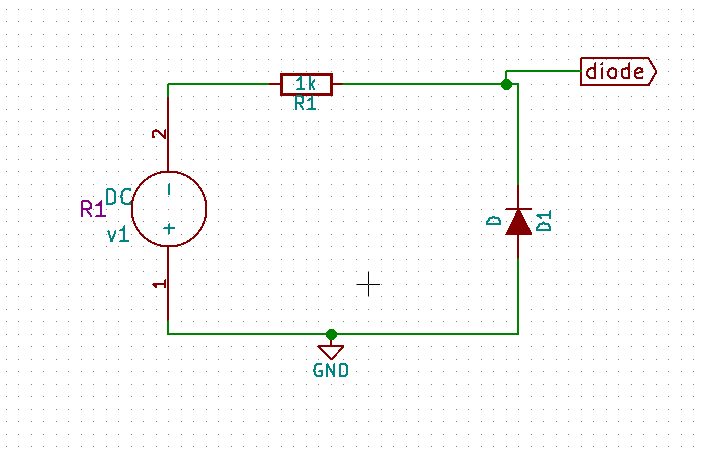
\includegraphics[width=0.8\textwidth]{diodeckt.png}
\caption{Schematic diagram for diode characteristics}
\label{diodeckt}
\end{figure}

\subsection*{PROCEDURE}

\subsubsection{Launch eSim}

\paragraph{}
 Launching eSim will take you to the dialog box which asks for the default workspace. Browsw the folders and set the wokspace location. It will finally end up in the eSim window shown in Figure \ref{LaunchWindow}.
\begin{figure}[h]
\centering
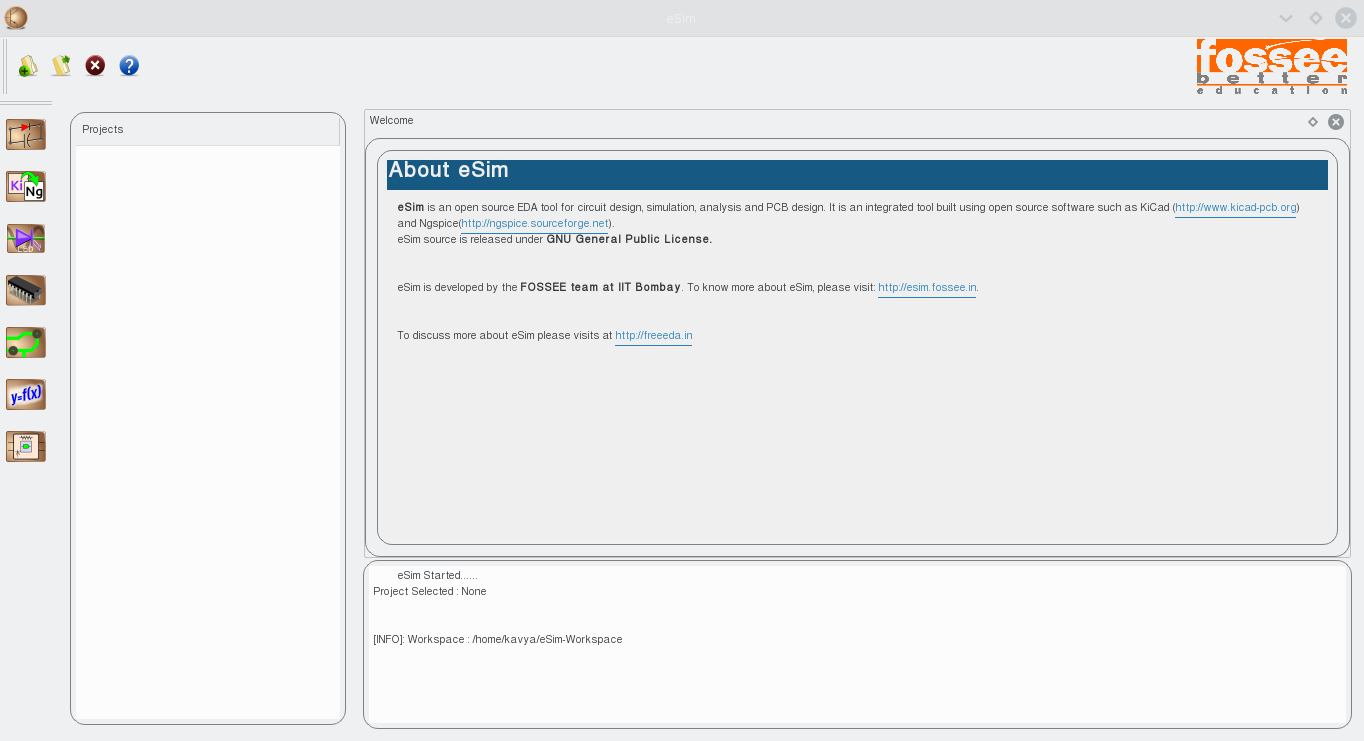
\includegraphics[width=0.8\textwidth]{LaunchWindow.png}
\caption{Launching eSim will take you to this window}
\label{LaunchWindow}
\end{figure}

\subsubsection{Create a New Project}

\paragraph{ } The new project is created by clicking the New icon on the
menubar. The name of the project is given in the pop up window as shown in Figure.\ref{newproject}.
\begin{figure}[h]
\centering
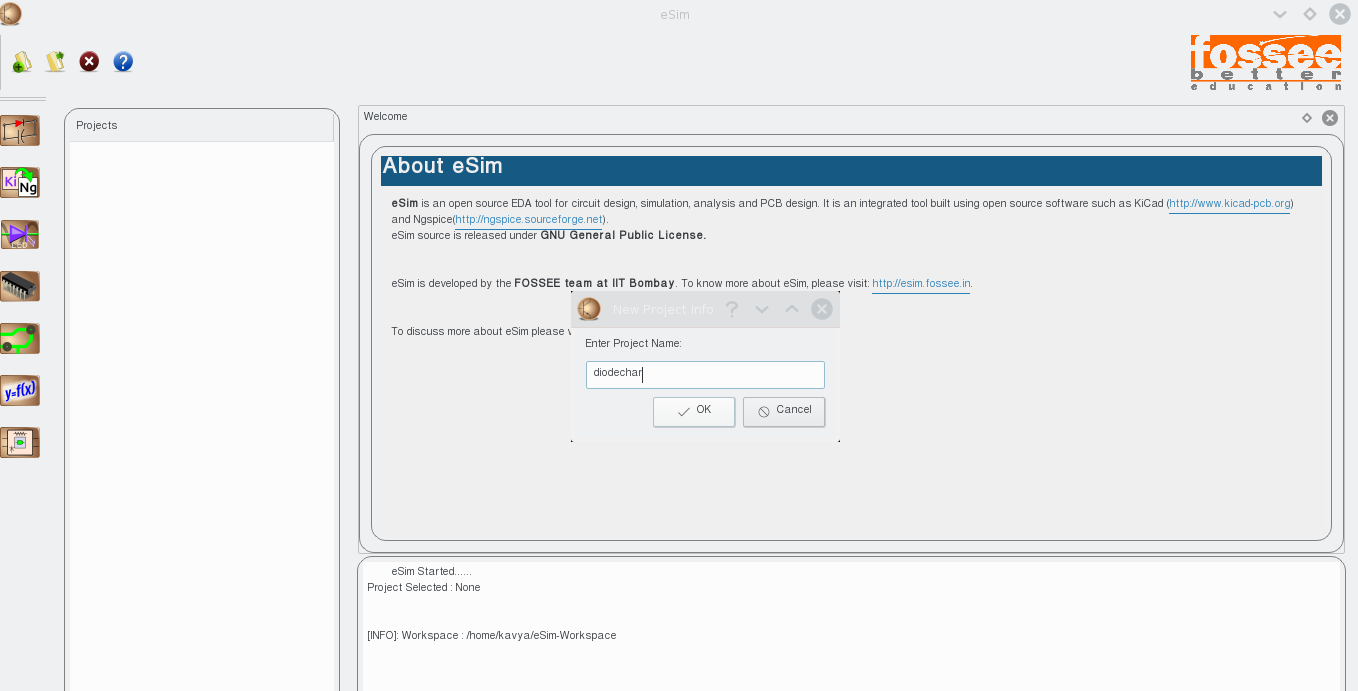
\includegraphics[width=\textwidth]{newproject.png}
\caption{Creating new project}
\label{newproject}
\end{figure}

\subsubsection{Create the Schematic}

\paragraph{}  To create the schematic, click the very first icon of the
left toolbar as shown in the Figure \ref{newschematic} .This will open KiCad Eeschema.


\begin{figure}[h]
\centering
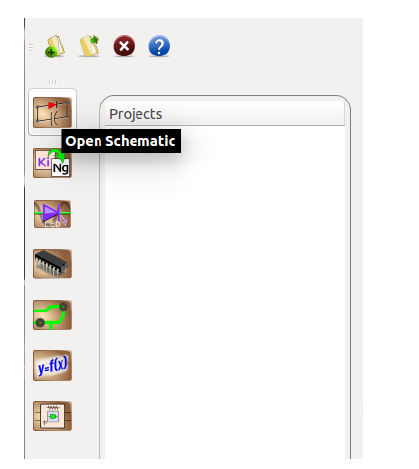
\includegraphics[width=0.5\textwidth, height=6cm]{newschematic.png}
\caption{Creating new schematic diagram}
\label{newschematic}
\end{figure}

To create a schematic in KiCad, we need to place the required components. See Figure \ref{kicad}

\begin{figure}[h]
\centering
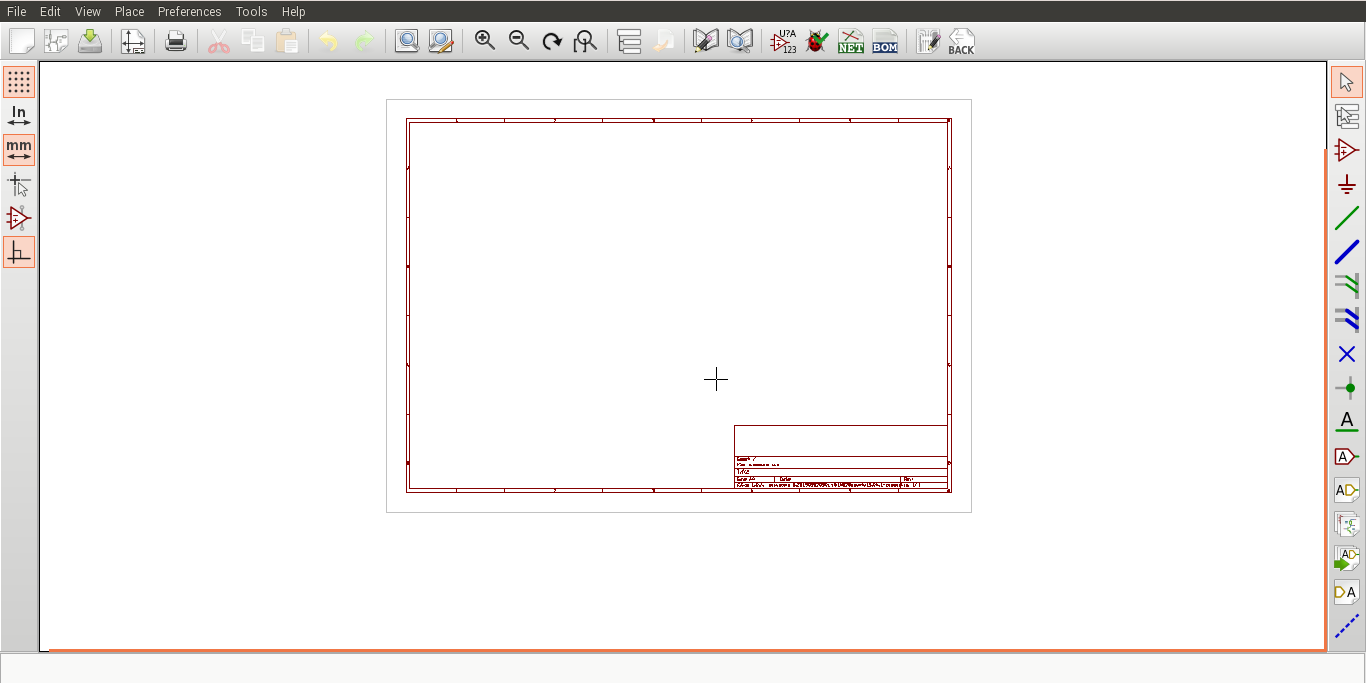
\includegraphics[width=0.5\textwidth, height=6cm]{kicad.png}
\caption{The Kicad Eeschema page}
\label{kicad}
\end{figure}

 Figure \ref{placecomponent}
shows the icon on the right toolbar which opens the component library. After all the required components of the simple RC circuit are placed, wiring is
done using the Place Wire option as shown in the Figure \ref{placewire}.Scroll up and down for zooming in and out.


\begin{figure}
\begin{minipage}{.5\textwidth}
  \centering
  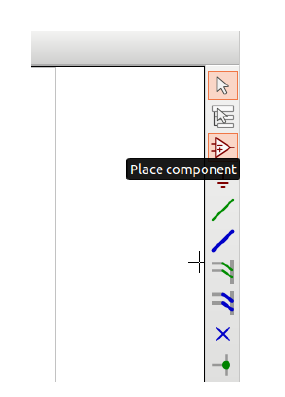
\includegraphics[width=\linewidth]{placecomponent.png}
  \caption{Place component icon}
  \label{placecomponent}
\end{minipage}%
\begin{minipage}{.5\textwidth}
  \centering
  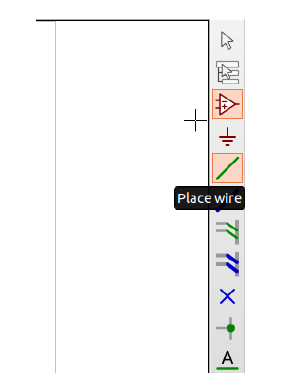
\includegraphics[width=\linewidth]{placewire.png}
  \caption{Place wire icon}
  \label{placewire}
\end{minipage}
\end{figure}


\paragraph{Placing the Components:} Normally all the components availbale in eSim can be chosen by left mouse click in the grid. The components are listed in different libraries. See Figure \ref{librarylist}.

\begin{figure}[h]
\centering
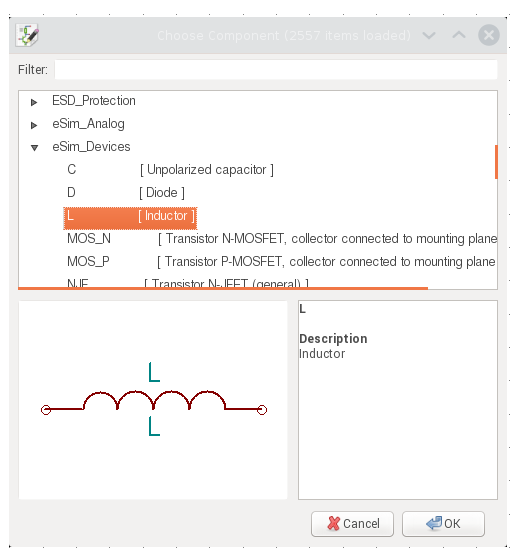
\includegraphics[width=0.5\textwidth, height=4cm]{librarylist.png}
\caption{The Kicad Libraries of components}
\label{librarylist}
\end{figure}

\begin{itemize}
\item
Choose DC source from eSim\_Sources
\item
Choose R from eSim\_Devices
\item
Choose D from eSim\_Devices
\item
Choose GND from power
\end{itemize}

Wire the components to get the circuit. A global label `diode' has been added to identify that node whose voltage will be later recorded and plotted.

\paragraph{Annotating the circuit:} Once the schematic diagram is completed, annotate it so that the `question marks' associated with the components are converted to meaningful numbers automatically. 
Select the resistor and edit its component value to 1k as shown in Figure \ref{editvalue}.

\begin{figure}[h]
\centering
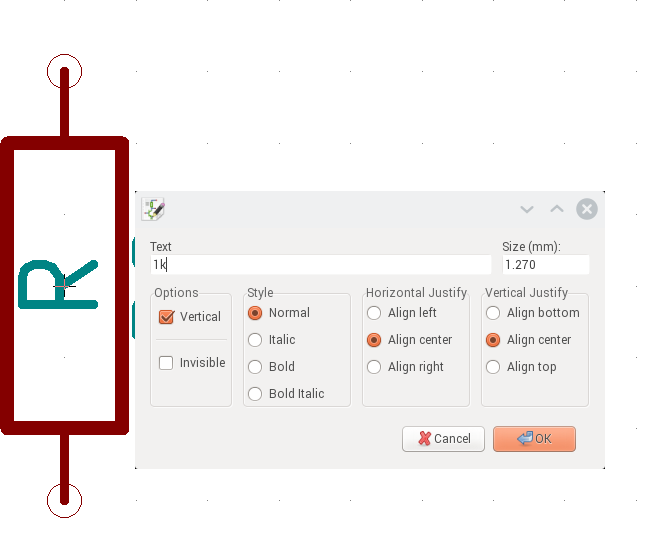
\includegraphics[width=0.5\textwidth, height=6cm]{editvalue.png}
\caption{Editing the value field of compenent R}
\label{editvalue}
\end{figure}

 Now we have the circuit diagram as shown in Figure \ref{diodeckt}.


\paragraph{Note:} If some libraries are found missing, you can add them from the `Preferences` menu by following the procedure: 

\begin{enumerate}
\item
Choose `Component Libraries' from Preferences menu.

\item
Click on the Add button on the top right side of the window.

\item
Choose the required libraries from `user/share/kicad/library' and click OK button

\end{enumerate}

\subsubsection{Create Netlist}


